
%%%%%%%%%%%%%%%%%%%%%%%%%%
\asubsection[A. Biek\"otter, D. Gon\c{c}alves, T. Plehn, M. Takeuchi, D. Zerwas]{Global analysis including the Higgs self-coupling}
\label{sec8:cubicetc}

% For convenience during refereeing: line numbers
%\linenumbers

%%%%%%%%%%%%%%%%%%%%%%%%%%%%%%%%%%%%%%%%%%%%%%%%%%%%%%%%%%%%%%%%%%%%%%

In record time Higgs physics has moved from a spectacular discovery of
a new particle to a systematic and comprehensive study of its
properties~\cite{Dawson:2018dcd}. 
One of the main goals of the physics program of a 27~\UTeV hadron 
collider 
is the measurement of the Higgs self-coupling in Higgs pair
production~\cite{Baur:2003gp,Kling:2016lay,Goncalves:2018yva,Homiller:2018dgu,Barger:2013jfa,Barr:2014sga},
testing for example a possible first-order electroweak
phase transition as an ingredient to
baryogenesis. 
We show that a 27~\UTeV hadron collider will for the first time 
deliver a meaningful measurement of this fundamental physics 
parameter~\cite{Biekotter:2018jzu}. \medskip

%%%%%%%%%%%%%%%%%%%%%%%%%%%%%%%%%%%%%%%%%%%%%%%%%%%%%%%%%%%%%%%%%%%%%%%
%\section{Higgs self-coupling} 
%\label{sec:gauge}
We perform a global study of Higgs physics at a 27~\UTeV hadron collider
using the effective dimension-6 Lagrangian~\cite{Brivio:2017vri} 
\begin{align}
\mathcal{L}_\text{eff} 
= & - \frac{\alpha_s }{8 \pi} \frac{f_{GG}}{\Lambda^2} \mathcal{O}_{GG}  
    + \frac{f_{BB}}{\Lambda^2} \mathcal{O}_{BB} 
    + \frac{f_{WW}}{\Lambda^2} \mathcal{O}_{WW} 
    + \frac{f_B}{\Lambda^2} \mathcal{O}_B 
    + \frac{f_W}{\Lambda^2} \mathcal{O}_W 
    + \frac{f_{WWW}}{\Lambda^2} \mathcal{O}_{WWW} \notag \\ 
  &  + \frac{f_{\phi 2}}{\Lambda^2} \mathcal{O}_{\phi 2} 
    + \frac{f_{\phi 3}}{\Lambda^2} \mathcal{O}_{\phi 3} 
    + \frac{f_\tau m_\tau}{v \Lambda^2} \mathcal{O}_{e\phi,33} 
    + \frac{f_b m_b}{v \Lambda^2} \mathcal{O}_{d\phi,33} 
    + \frac{f_t m_t}{v \Lambda^2} \mathcal{O}_{u\phi,33} \notag \\
  & + \text{invisible decays} \; .
\label{eq:ourleff}
\end{align}
%
with the operators defined in Ref.~\cite{Butter:2016cvz}, 
and specifically
%
\begin{align}
\mathcal{O}_{\phi 2} = \frac{1}{2} \, \partial^\mu (\phi^\dagger \phi) \partial_\mu (\phi^\dagger \phi)  
\qquad \qquad
\mathcal{O}_{\phi 3} = -\frac{1}{3} \, (\phi^\dagger \phi)^3 \; ,
\label{eq:ope23}
\end{align}
%
describing a modified Higgs potential. In addition, we include invisible 
Higgs decays as an additional contribution to the total width or, equivalently, 
the invisible branching ratio.
%------------------------------------------------
\begin{figure}
\centering
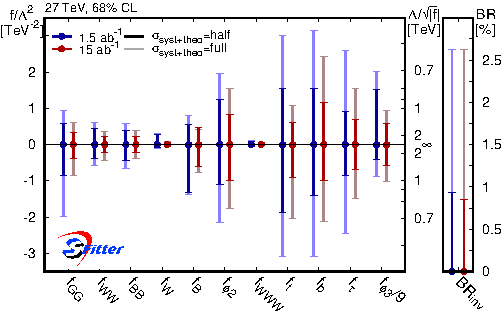
\includegraphics[width=0.65\textwidth]{\main/section8/plots/HiggsHELHCtheo2_hall2_BR_aspect_logo}
\caption{Result from the global Higgs analysis in terms of dimension-6
  operators. All limits are shown as profiled over all other Wilson
  coefficients. Figure from Ref.~\cite{Biekotter:2018jzu}.}
\label{fig:d6}
\end{figure}
%------------------------------------------------

The self-coupling with its unique relation to the Higgs potential is
not yet included in most global analyses of SM-like Higgs 
couplings~\cite{Ellis:2018gqa,Alves:2018nof,Biekotter:2018rhp}
because of the modest reach of the LHC Run~II.  
However, for a 27~\UTeV
collider with an integrated luminosity of $15~\iab$ we quote the
expected reach~\cite{Goncalves:2018yva}
%
\begin{align}
\frac{\lambda_{3H}}{\lambda_{3H}^\text{(SM)}}
=\begin{cases} 
1 \pm 15\% &  68\%~\text{C.L.} \\
1 \pm 30\% &  95\%~\text{C.L.} 
\end{cases}
\label{eq:reach_lam}
\end{align}
%
We can translate this range into the conventions of
Eq.\eqref{eq:ourleff} assuming that the underlying new physics
only affects $\mathcal{O}_{\phi 3}$,
%
\begin{align}
V = \mu^2 \; \frac{(v+H)^2}{2} 
  + \lambda \; \frac{(v+H)^4}{4} 
  + \frac{f_{\phi 3}}{3 \Lambda^2} \; \frac{(v+H)^6}{8} \; .
\end{align}
%
The reach of the dedicated one-parameter self-coupling
analysis becomes
%
\begin{align}
\lambda_{3H} 
= \lambda_{3H}^\text{(SM)}
  \left( 1 + \frac{2 v^2}{3 m_H^2} \; \frac{f_{\phi 3} v^2}{\Lambda^2} \right) 
\qquad \text{and} \qquad
\left| \frac{\Lambda}{\sqrt{f_{\phi 3}}} \right| \gtrsim
\begin{cases}
1~\text{\UTeV} &  68\%~\text{C.L.} \\
700~\text{\UGeV} &  95\%~\text{C.L.} 
\end{cases}
\label{eq:reach_d6}
\end{align}

Our global analysis containing all operators in Eq.\eqref{eq:ourleff}
is based on a re-scaling of the number of signal and background events 
in the 8~\UTeV analysis~\cite{Corbett:2015ksa} to 27~\UTeV, assuming two
experiments. For the invisible Higgs searches we use an in-house extrapolation of
the WBF analysis~\cite{Eboli:2000ze} from Ref.~\cite{Biekotter:2017gyu} to 27~\UTeV.  
Because the effective Lagrangian of Eq.\eqref{eq:ourleff} includes new
Lorentz structures, especially valuable information comes from the
kinematic distributions~\cite{Englert:2015hrx,Corbett:2015ksa} listed in Tab.~\ref{tab:distr}.
%\textit{probing interactions with a large momentum flow}.
They are particularly relevant for our analysis of the Higgs self-coupling,
where the full kinematic information from Higgs pair production encoded in
the $m_{HH}$ distribution allows us to separate the effects of
$\mathcal{O}_{\phi 2}$ and $\mathcal{O}_{\phi  3}$~\cite{Kling:2016lay,Goncalves:2018yva}.
Following Refs.~\cite{Bizon:2016wgr,Maltoni:2017ims,DiVita:2017eyz} we neglect the loop effects
of $\mathcal{O}_{\phi 3}$ on single Higgs production, because they will
hardly affect a global Higgs analysis.  
\medskip

%------------------------------
\begin{table}[t!]
\centering
\begin{tabular}{lrrr}
\toprule
channel  & observable & \# bins & range [\UGeV] \\
\midrule
$WW \rightarrow (\ell \nu)(\ell \nu)$          & $m_{\ell\ell'}$ & $10$ & $0-4500$\\
$WW \rightarrow (\ell \nu)(\ell \nu)$          & $p_T^{\ell_1}$ & $8$ & $0-1750$\\
$WZ \rightarrow (\ell \nu)(\ell \ell)$          & $m_T^{WZ}$ & $11$ & $0-5000$\\
$WZ \rightarrow (\ell \nu)(\ell \ell)$          & $p_T^{\ell\ell}$ ($p_T^Z$) & $9$ & $0-2400$\\
WBF, $H\rightarrow \gamma\gamma$          & $p_T^{\ell_1}$ & $9$ & $0-2400$\\
$VH \rightarrow (0\ell) (b \bar{b})$ & $p_T^V$ & $7$ & $150-750$\\
$VH \rightarrow (1\ell) (b \bar{b})$ & $p_T^V$ & $7$ & $150-750$\\
$VH \rightarrow (2\ell) (b \bar{b})$ & $p_T^V$ & $7$ & $150-750$\\
$HH \rightarrow (b \bar{b}) (\gamma \gamma)$, $2j$ & $m_{HH}$ & $9$ & $200-1000$ \\
$HH \rightarrow (b \bar{b}) (\gamma \gamma)$, $3j$ & $m_{HH}$ & $9$ & $200-1000$ \\
\bottomrule
\end{tabular}
\caption{Distributions included in the analysis. The number of bins
includes an overflow bin for all channels. Table from Ref.~\cite{Biekotter:2018jzu}.}
\label{tab:distr}
\end{table}
%------------------------------


In Fig.~\ref{fig:d6} we show the expected reach for the global 
Higgs analysis in terms of dimension-6 operators for a 27~\UTeV LHC upgrade. 
For all measurements we assume the SM predictions,
which means that our best-fit points will always be the SM values.
To illustrate the importance of precision predictions we
will show results with the current theory uncertainties as well as an
assumed improvement of theory and systematics by a factor two.
Asymmetric
uncertainty bands arise because of correlations, but also reflect
numerical uncertainties.  Different colours correspond to assumed
integrated luminosities of $1.5~\iab$ and $15~\iab$.  
Most of the effective operators
benefit from an increased statistics, because larger luminosity
extends the reach of kinematic distributions, which in their tails are
always statistically limited. In contrast, the Yukawa couplings
$f_{b,\tau}$, which do not change the Lorentz structure, are mostly
limited by the assumed systematic and theory uncertainties.
Consequently, the reach for operators which modify the Lorentz
structure of some Higgs interaction exceeds the reach for the
Yukawa-like operators or the reach for the operator $\mathcal{O}_{\phi 2}$,
which introduces a wave function renormalisation  for the Higgs field
and only changes the kinematics of Higgs pair production. 


%------------------------------------------------
\begin{figure}[t!]
\centering
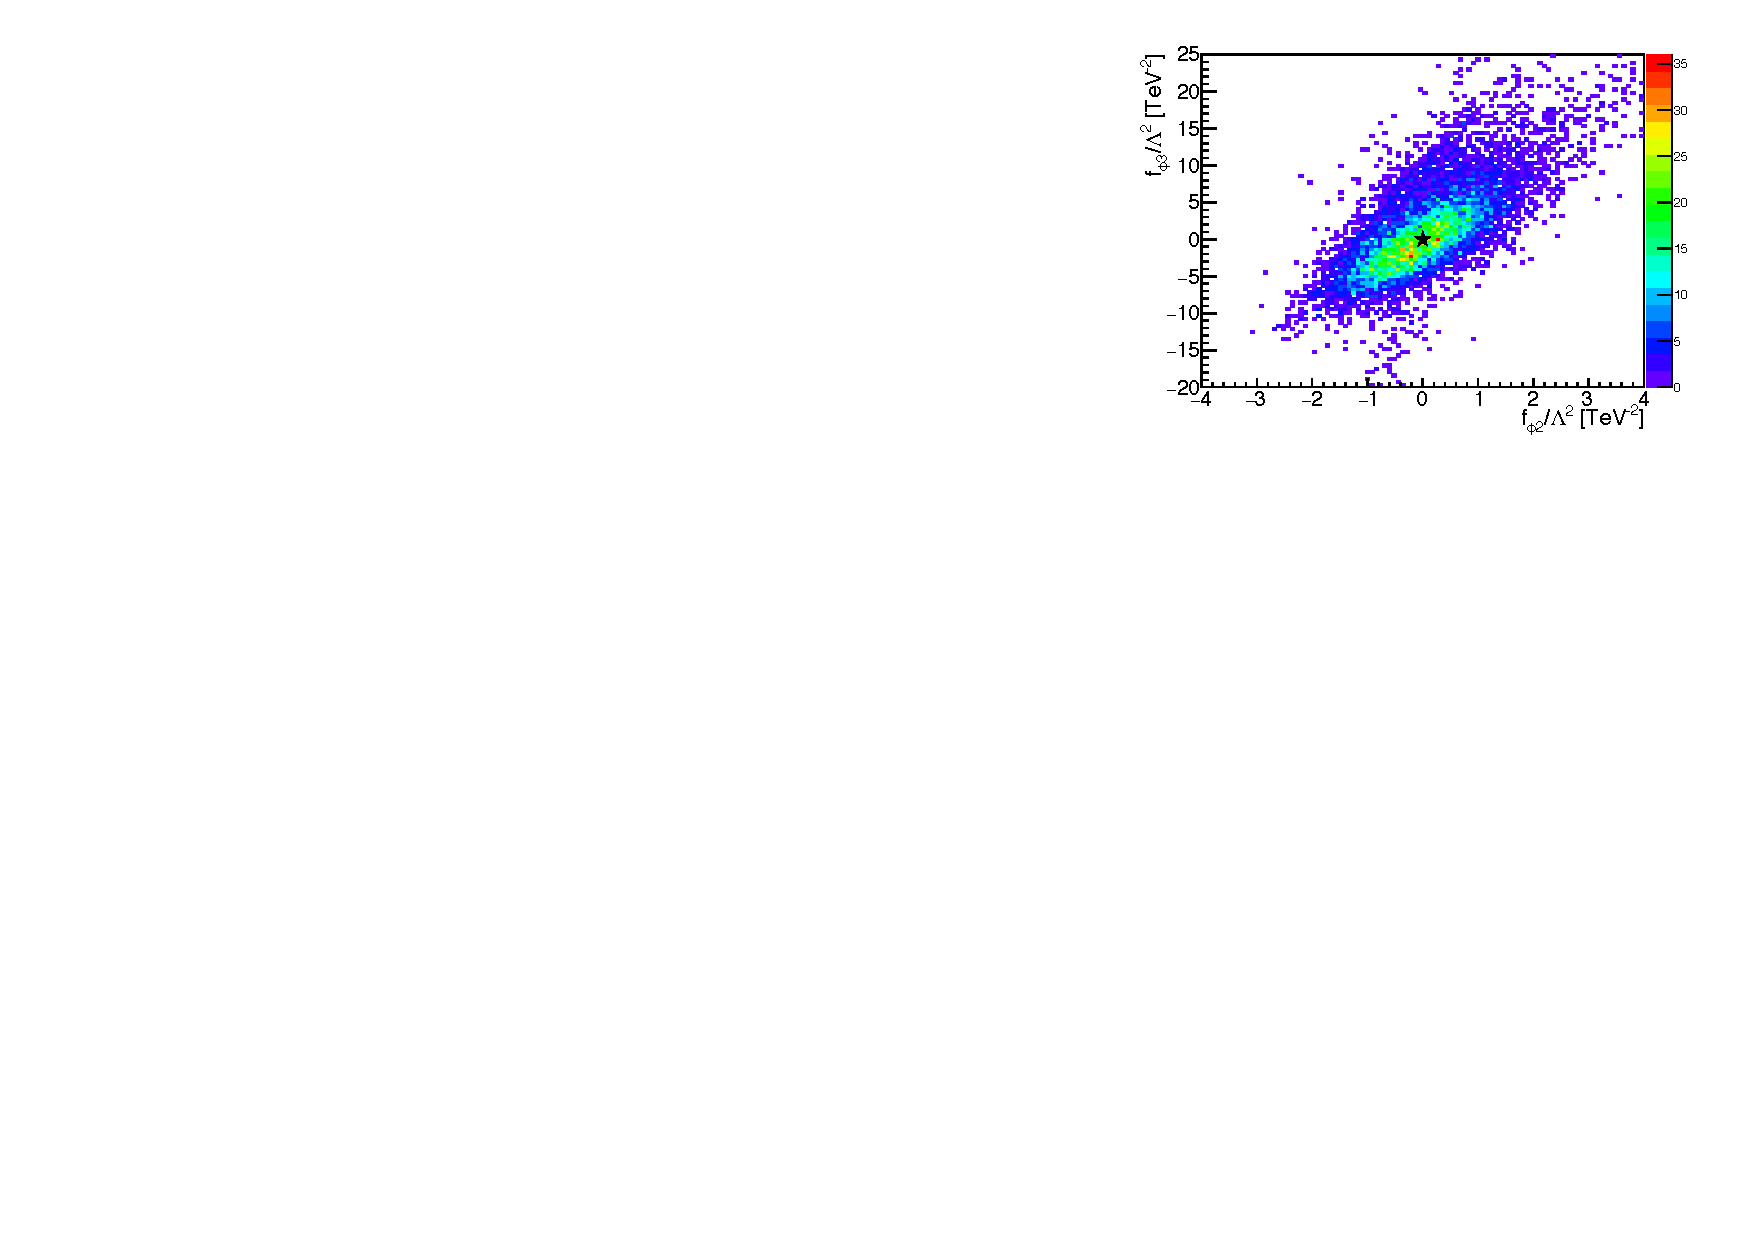
\includegraphics[width=0.5\textwidth]{\main/section8/plots/corr_half_15ab_nov}
\caption{Correlations between the leading operators describing Higgs
  pair production. Figure from Ref.~\cite{Biekotter:2018jzu}.}
\label{fig:corr}
\end{figure}
%------------------------------------------------
For the operator $\mathcal{O}_{\phi 3}$, which modifies the Higgs potential
as part of a global analysis, we find the limits
%
\begin{alignat}{9}
\frac{\Lambda}{\sqrt{|f_{\phi 3}|}} &> 430~\text{\UGeV}
&\qquad \text{68\% C.L.} \notag \\
\frac{\Lambda}{\sqrt{|f_{\phi 3}|}} &> 245~\text{\UGeV}
\quad (f_{\phi 3} >0)
\quad \text{and} \quad 
\frac{\Lambda}{\sqrt{|f_{\phi 3}|}} > 300~\text{\UGeV}
\quad (f_{\phi 3} <0) 
&\qquad \text{95\% C.L.} 
\label{eq:reach_d6_3}
\end{alignat}
%
These limits are diluted from the one-parameter analysis quoted in
Eq.\eqref{eq:reach_d6}, largely because of the combination with
$\mathcal{O}_{\phi 2}$. We can directly compare the
effects from $\mathcal{O}_{\phi 2}$ and $\mathcal{O}_{\phi 3}$ for similar values of
$f/\Lambda^2$ as a function of the momentum flowing through the
triple-Higgs vertex or $m_{HH}$. In that case we find that the
momentum dependence in $\mathcal{O}_{\phi 2}$ matches the effects from
$\mathcal{O}_{\phi 3}$ for $m_{HH} \gtrsim 1$~\UTeV, with either relative
sign. 
In Fig.~\ref{fig:corr} we show 
the correlation between $\mathcal{O}_{\phi 2}$ and $\mathcal{O}_{\phi 3}$
which is not
accounted for in the usual Higgs pair analyses.
The global analysis obviously
reduces the reach for the Higgs self-coupling modification compared to
a one-parameter analysis, but still indicates that a 27~\UTeV hadron
collider will for the first time deliver a meaningful measurement of
this fundamental physics parameter. 

